\documentclass[a4paper]{article}

%% Language and font encodings
\usepackage[english]{babel}
\usepackage[utf8x]{inputenc}
\usepackage[T1]{fontenc}
\usepackage{graphicx}
\usepackage{caption}
\usepackage{subcaption}
\usepackage{eurosym}
\usepackage{multirow}
\usepackage{footnote}
\usepackage{listings}
\usepackage{color}
\usepackage{pdfpages}

%% Sets page size and margins
\usepackage[a4paper,top=3cm,bottom=2cm,left=3cm,right=3cm,marginparwidth=1.75cm]{geometry}

%% Useful packages
\usepackage{amsmath}
\usepackage{graphicx}
\usepackage[colorinlistoftodos]{todonotes}
\usepackage[colorlinks=true, allcolors=blue]{hyperref}
\begin{document}

\begin{titlepage}

\newcommand{\HRule}{\rule{\linewidth}{0.5mm}} % Defines a new command for the horizontal lines, change thickness here

\center % Center everything on the page
 
%----------------------------------------------------------------------------------------
%	HEADING SECTIONS
%----------------------------------------------------------------------------------------

\textsc{\LARGE Ecole Polytechnique de Bruxelles}\\[1.5cm] % Name of your university/college
\textsc{\large Johnston Lab Internship}\\[0.5cm] % Minor heading such as course title

%----------------------------------------------------------------------------------------
%	TITLE SECTION
%----------------------------------------------------------------------------------------

\HRule \\[0.4cm]
{ \huge \bfseries User Guide Thermography}\\[0.4cm] % Title of your document
\HRule \\[1.5cm]
 
%----------------------------------------------------------------------------------------
%	AUTHOR SECTION
%----------------------------------------------------------------------------------------

\begin{minipage}{0.4\textwidth}
\begin{flushleft} \large
\emph{Author:}\\
Maxime \textsc{Verstraeten} % Your name
\end{flushleft}
\end{minipage}
~
\begin{minipage}{0.4\textwidth}
\begin{flushright} \large
\emph{Supervisors:} \\
Jamie \textsc{Johnston}\\[0.3cm] % Supervisor's Name
\end{flushright}
\end{minipage}\\[2cm]

% If you don't want a supervisor, uncomment the two lines below and remove the section above
%\Large \emph{Author:}\\
%John \textsc{Smith}\\[3cm] % Your name

%----------------------------------------------------------------------------------------
%	DATE SECTION
%----------------------------------------------------------------------------------------

{\large \today}\\[2cm] % Date, change the \today to a set date if you want to be precise

%----------------------------------------------------------------------------------------

\vfill % Fill the rest of the page with whitespace

\end{titlepage}


\noindent\rule{\textwidth}{1pt}

\tableofcontents

\newpage

\listoffigures

\newpage



\section{Introduction}
This user guide intends to provide the user an understanding of the Thermography device developped at Johnston Lab as well giving the reader useful indications for troubleshooting.

Note: as of 3rd of September 2019, the device has shown extremely encouraging results on human but is not working on mice. This due to the smaller nostrils, smaller volume of air and smaller temperature delta.

Note2: The workflow, thoughts, issues, ... for this project are discussed in my OneNote.

The latest updates are available on my Github: \url{https://github.com/maverstr/Thermography}

\section{Objective}
The device purpose is to provide a visualisation of the respiration of a mouse during 2-photon imaging.

The idea is to implement an infrared thermography system allowing for respiration cycle detection by detecting the cold air flow coming to the nostrils when the mouse is breathing in and hotter air coming out at the expiration. 

This kind of device already exists (see IR thermography-based monitoring of respiration phase without
image segmentation - K. Mutlua,b, J. Esquivelzeta Rabella,b, P. Martin del Olmod, S. Haeslera,b,c,d ) but uses high-performance and expensive cameras (FLIR A325sc with 50 µm lens, 60 fps, 320 × 240 pixels, about 11 000£). 

The device allow to obtain similar results with a much more inexpensive design and equipment, easily reproducible and open-source.

To do so, I use the MLX90640 camera (32x24 pixels resolution, 32Hz max, 30£), a LCD display ILI9341 and an ESP32 as a microcontroller.

\section{Hardware}
\subsection{Infrared camera}
The camera used is the MLX90640. It comes on a small breakboard with 4 usable pins among 5. The communication protocol used is I2C.
The pins are:
\begin{itemize}
    \item VDD: 3.3V or 5V (3.3V on the device)
    \item GND: ground
    \item SDA: Signal Data
    \item SCL: Signal Clock.
\end{itemize}


\subsection{LCD Display}
The LCD Display is used to get the camera signal and help the user to place the camera correctly in front of the nostrils.
The display used in the device is the TFT ILI9341. It can be controlled either with SPI mode or 8-bit parallel. Because of the multiple pins required on the microcontroller for buttons, switches, camera and display, the SPI mode is used. The parallel mode would be faster but requires 8 more pins.

Note that some jumpers must be soldered to choose the correct mode.

This display also comes with a resistive touchscreen. This allows to crop the image in order to reduce the number of pixels which must be computed and get a faster refresh rate.

\subsection{Microcontroller}
An ESP32 has been chosen as the microcontroller as it is fast, reliable, available as a devkit and has a high number of pins among some ADC and DAC pins.

Note: when using the Arduino IDE to flash the ESP, the boot button must be held down during the communication. A simple workaround is to solder a 10µF capacitor between GND and pin EN.


\subsection{Enclosure}
The device comes with an enclosure.
The display is on top of it with 3 pushbuttons and toggleswitch. A micro USB connector on the side is required for power as well as to flash the µC and a BNC connector outputs the analog signal of the breathing.
The camera is linked to the enclosure via a 4-core connector and a cable.


\section{Software}
The whole code is available on my github (https://github.com/maverstr/Thermography)

\subsection{Libraries}
The µC is flashed through the Arduino IDE. The ESP32 core is therefore required. (https://github.com/espressif/arduino-esp32).

Multiple libraries are required and some of them have been modified to use with the device. Most of them are available as part of my release on Github.

\begin{itemize}
    \item mlx90640 API (reworked)
    \item mlx90640 I2C Driver (reworked)
    \item RunningStat (for standard deviation running computation)
    \item TFT eSPI (reworked)
    \item Touchscreen
    \item driver/dac
    \item Wire.h
    \item SPI.h
\end{itemize}


\subsection{How does it work?}
As usual in a microcontroller code, comes the declaration of all the variables and functions. Then comes a setup and finally the loop.

\subsection{Setup}
The setup initalizes all the interrupt pins and the required pull-ups then starts a Serial at 500,000bauds and an I2C communication at 400kHz.
The µC then tries to communicate with the camera and initialize it. Time to also extract the EEPROM calibration data through an EEPROM dump. This is necessary for this step to be done at 400kHz max.
Once the EEPROM is released, the I2C is set 1MHz (fast-mode plus).

At the end of the setup, a reference frame is taken and a calibration is performed.

\subsection{Loop}
The loop is divided in 3 main parts:
\subsubsection{Temperature Reading}
This mode is the most precise one and can be toggled to via the toggleswitch on top of the enclosure. It is however the slowest.
\subsubsection{Raw Reading}
This is the most important mode as the data will be gathered from there. 

Firs, we check a specific bit (bit 2) at 0x8000 indicating if new data is available in the RAM of the camera (meaning a new acquisition has been done).
This avoid running computation on data already done before and allows to be ready to immediately work on new data.
This bit must be manually reset to 0 when starting a new computation.

The camera stores data in 32x24 (768) registers. We therefore go through each of them, or only several depending on the cropping settings. The I2C buffer allows to get 32bytes of data in one read so we work on one row at a time.

First, as the data is unsigned int, a gain correction is performed (i.e. if value > 32767, value - 65536).

Now, we can use the data from the EEPROM and ambient temperatures to correct these values, which makes them floating point and is required to have a proper temperature accuracy. However,regarding the computation speed. The ESP32 is indeed slow with float but quite fast with integers. It is therefore more interesting to keep the values as integers. Corrections not required when comparing frames to get the trend as the same correction is applied to the same pixel every frame. We can therefore avoid these corrections when comparing the same pixels on different frames. This however, intrinsically creates a "reference frame".

Integrating a derivative gives the original variable but without a constant. Again, this is interesting in our case as we are only interested in relative temperature difference.
In the discrete word, integrate a derivation is the same as comparing 2 frames and sum the delta for every comparison.
We therefore have several arrays containing the actual frame, the last frame, the derivative and the integration (the whole sum).

The values can either be sent further as they are or averaged over a few frames (rolling average).
They can also be changed through a look-up-table for histogram equalization.

These values can then be mapped to 8-bit values (for DAC output and for LCD 8bit grayscale representation) and to do so, we use the maximum and minimum values obtained from a Calibration (see subsection \ref{calibration}).

The analog output is the average of the pixels inside the ROI. This ROI can be either the whole cropped region or only the pixels which a standard deviation above a certain threshold inside the cropped region. 

\subsubsection{Interrupt and Serial handling}
Whenever an interrupt is triggered, a corresponding flag is set. At the end of each loop, we check the values of each flag and relevant operations is performed.

Same thing if bytes are waiting in the Serial buffer (used mainly for debugging purposes or added functionalities).


\subsection{Calibration}
\label{calibration}
A calibration is performed at the end of the setup and on request with a pushbutton. The calibration takes 64 frames in a row and keeps the maximum and minimum pixel values of these frames. This gives a range on which to map the values. The range is in practice reduced by 30\% to have a higher demarcation between high and low values and avoid aberrant range. Moreover, the values higher than the range are set to max range.

\subsection{Reference Frame}
Because intrinsically comparing frames makes the first frame a "reference", this reference can be reset by setting the sum (integration of the derivatives) to zero for every pixel.
It is therefore important to put the camera in front of an uniform background when taking a new reference frame (improvement: one could think about adding a shutter that closes when taking a new reference). 

If it is done in front of the nostrils, this will simply remove the facial background. This can sometimes improve the contrast for the nostrils but ideally you want the reference frame to be taken exactly at the point of end of expiration which although easy on humans can be difficult on mice.

\subsection{Histogram}
In order to improve the contrast of both the image and the analog output, an histogram analysis is done on calibration and a look-up-table for histogram equalization is created. This makes the image more noisy and harder for a human to see what is in front of the camera but it can improve the contrast of the data.

\subsection{Standard Deviation}
A running standard deviation analysis is performed on each pixel over undefined time. This allows to get the data only from pixels which show a high variance (the nostrils typically) and should give more accurate data but the threshold needs fine-tuning. The standard deviation table can be reset through a specific command.

\section{How to use?}
The device must be powered through the USB connector on the side of the enclosure.
The toggleswitch will switch between temperature reading and raw reading. To get a clear view of what is in front of the camera, the temperature reading is preferred but for data retrieval, the device must be set to raw reading mode.

When powered, the device will take 2-3 seconds to calibrate itself. You ideally want to orient the camera to an uniform background at this point. 

The FOV being narrow, the camera must be placed close (i.e. withing 2-3 cm) to the nostrils.
On both modes you should be able to see human nostrils.

When satisfied with the camera placement, you can start cropping the screen. To do so, press the green button on the screen. When pressed it should turn blue and you can point on the screen to set the first corner of the cropping. Do the same with the purple one. A square is drawn on the image. If satisfied, press the yellow button to validate.

TIP: you can also "uncrop" by drawing the square out of bounds of the ROI.

You can then press the button to take a new calibration and, if needed, a new reference frame. Rolling average can be toggled through another button.

The analog signal will be sent to the BNC connector and can be seen with an oscilloscope.

\section{Expected results}
When using the device on human nostrils, the display should show black and purples pixels on the nostrils. (purple simply means below the minimum calibration values and is useful to quickly see if the camera is correctly placed).

The oscilloscope should show an analog signal from 0V to 3.3V. In practice, the range is more 600mV to 2.8V.

\section{Electronic schematics}
The schematic is pretty simple.
The ESP32 got his own socket on the PCB.
Buttons and switches are linked to ground and digital pull-ups.
RC Circuit low-pass on the output and RC circuit low-pass to hardware debounce the switch.
There are also two supply decoupling capacitors.
A 5V pin is free to use as well as multiple ground pins.

The pin headers for the camera should be connected to the 4-core connector and the headers for the display should be directly connected. They are both sequenced in the good order (meaning every wire side-by-side on the PCB should be side-by-side on the camera and display).
\begin{figure}
    \centering
    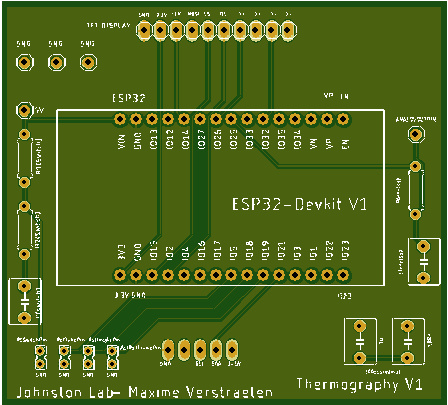
\includegraphics[width = 12cm]{images/PCBViewer.png}
    \caption{PCB View}
    \label{fig:PCBView}
\end{figure}

\begin{figure}
    \centering
    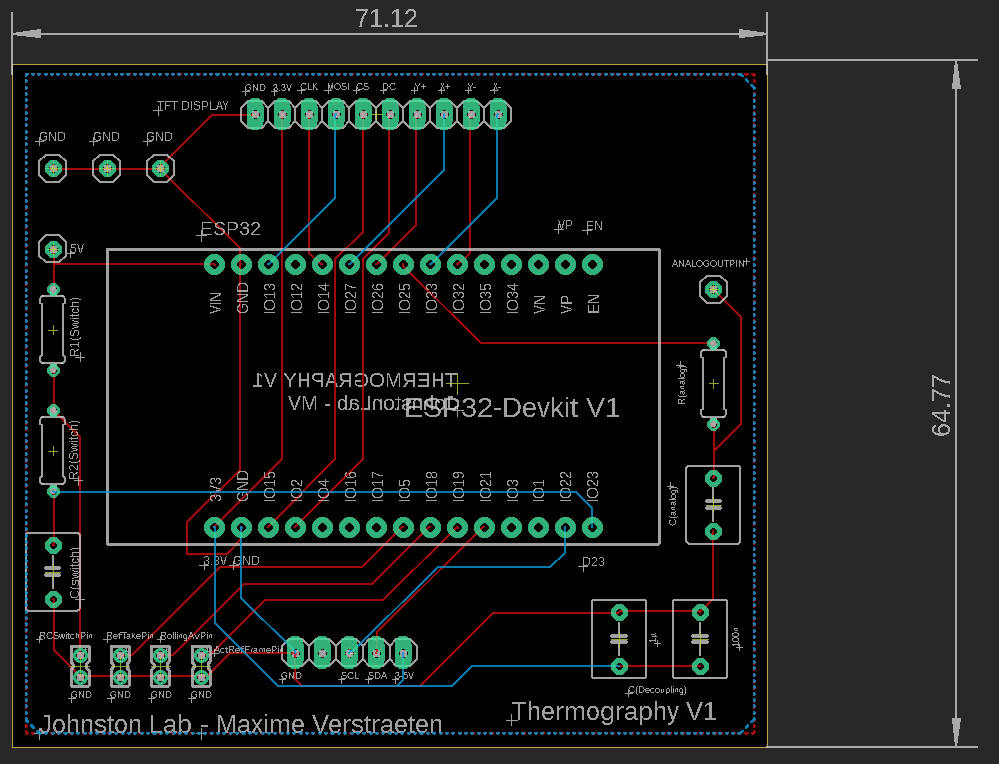
\includegraphics[width = 12cm]{images/BoardView.PNG}
    \caption{PCB Design}
    \label{fig:BoardView}
\end{figure}


The schematic can be seen in subsection \ref{schematic}.

\section{Troubleshooting}
\subsection{Buttons not working}
Check that the wires connected to the buttons are still there and haven't been torn apart (usually ground and digital pull-up).
\subsection{Touchscreen not working}
Make sure that the 4 wires for the touchscreen are well connected. If the touchscreen works but doesn't interact where you actually touch the screen, the order of the cables might be reversed.
\subsection{}

\section{Other tools}
\subsection{Processing3 data recording}
A script in Java (Processing3) has been written to be able to record the data from the Serial output into Excel files.
The script is available on Github.

To use it, simply activate the Serial Output in the ESP32 code and make sure to end each frame with a "@" character.  

\subsection{Python visualisation}
I've made a script that allows to visualize the results from the Processing3 recording. Simply convert the .csv files into .txt files and use Notepad++ to search and replace: "" by nothing. Then call the file raw.txt and launch the Python script.

\begin{figure}[h!]
    \centering
    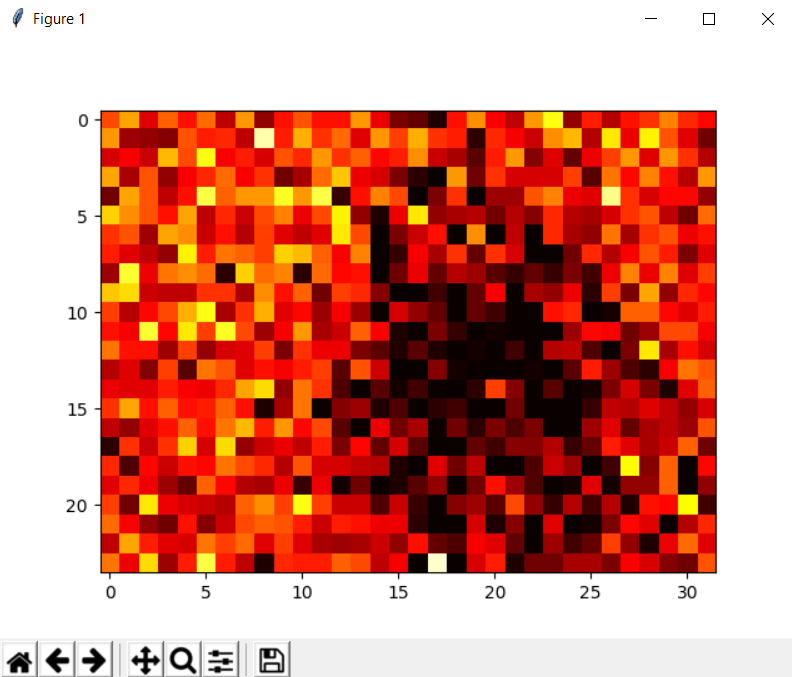
\includegraphics[width = 10cm]{images/python.PNG}
    \caption{Python visualisation}
    \label{fig:python}
\end{figure}


\subsection{MLX90614}
A few tries have been done with an MLX90614.
The datasheet wasn’t really detailed concerning the refresh rate. I knew I couldn't expect more that 8Hz in SMBus mode (similar to i2c) but a PWM mode is available and the increase in accuracy (and therefore sensitivity) was worth the try.

The connection is pretty simple : 3.3V on VDD, GND on VSS and SCL and SDA to respective pins. The SMBus mode works correctly although the precision in non thermal equilibrium is somehow a bit wrong.
Note that pull-up resistors are needed on SCL and SDA.

The refresh rate is capped just below 8Hz…

To switch to PWM mode, a value must be changed in the EEPROM of the sensor. Address: 0x22, value : 0b111
Then the sensor can be unplugged and replugged or put in sleep mode and then wake it up. The PWM signal is available on SDA pin and SCL should be pulled high.
To switch back to SMBus mode (necessary to change other EEPROM values), the SCL must be kept low for a few milliseconds then back to microcontroller SCL. Once back in SMBus, the register value can be changed again to 0b000 otherwise on next POR it reverts back to PWM mode.

The temperature ranges are set in addresses 0x20 (max) and 0x21 (min). The values are entered in Kelvin x100 (i.e. 20°C = 29325 = 0x728D

The config register can be changed (0x25) to reduce the settle time.

Unfortunately, the sensor does not seem to be able to catch the respiration and is too slow.

\section{Improvements}
\subsection{PCB}
Regarding the electronic circuit:
\begin{itemize}
    \item Add a 10µF capacitor between EN and GND to allow easy flashing of the ESP32 on the PCB instead of soldering it to the ESP32 directly.
    \item Add external pull-ups for SDA and SCL instead of on the camera directly.
    \item Increase Hole size and screw the PCB on the enclosure instead of gluing it.
    \item Add a GPIO pin header for testing purposes (e.g.  GPIO4). It allows for example to trigger the oscilloscope on that channel and put the pin to digital high and low at specific moments in the code. Allows easy understating of the timing and dynamics of the code.
\end{itemize}

\subsection{Lens}
To improve the resolution of the camera and be able to use it on mice, adding an IR lens might help.
Using Wien's displacement law for black bodies and the datasheet extreme temperatures to which the camera is sensitive the wavelength that we are interested in should be between 5µm and 12.5µm.

For the mouse range of temperature, the wavelengths are around 9.2µm and 10.7µm.

\subsection{I2C push-pull}
The I2C camera communication can go as fast as 1MHz (Fast-mode plus). At first, the actual frequency could not go higher than 400kHz. This is because the internal pull-ups of the ESP32 chip are too weak to be able to sustain a fastModePlus (1Mhz) frequency. 


\textit{ESP32 datasheet: The I²C interfaces support: • Standard mode (100 Kbit/s) • Fast mode (400 Kbit/s) • Up to 5 MHz, yet constrained by SDA pull-up strength }

Therefore to increase the actual frequency, I used external pull-ups. (I2C being open-drain, we need pull-ups to drive the pins high).
This is however a trade-off (http://www.ti.com/lit/an/slva689/slva689.pdf) between power-consumption and speed.
The lower the resistor value, the stronger the pull up and therefore the rising edges of the I2C are fast, leading to a high I2C frequency. However if the pull-ups are too strong, there is not enough current (the transistor cannot sink enough current) for the data to get to digital low before a new clock arise. This leads to corrupted communication.

\textit{Digital outputs have a specified ability to source or sink current. If your output could sink 5 mA and the output was connected through a pull-up to 5 V and then set to 0, you would need a minimum of 1k resistance. If you use less than 1k, the output will not be able to sink enough current to pull the pin all the way down to 0V. If you use a bigger value, like 10k, then the pin only has to sink 0.5 mA, which is much less than it's rating.  (https://electronics.stackexchange.com/questions/1849/is-there-a-correct-resistance-value-for-i2c-pull-up-resistors)
}

There is therefore also a trade-off between speed and reliability and maximum and minimum resistor values for a set frequency.


Some pictures of the I2C communication is available on OneNote.

On the pictures we can see that the clock signal rising edges are slow (similar to an RC) which makes the I2C slow.

In fact, the ESP32 waits to actually "see" the high bit when setting a high output. That allows I2C slaves to keep a clock at low state to slow the I2C down. This process is called I2C clock-stretching.
A solution to increase the speed is therefore to drive the clock in push-pull mode instead of open drain. We can probably do that as the mlx90640 camera does not do any clock stretching (according to its datasheet), there are no other slaves on the same I2C bus and no other masters that could drive the clock.

(This is also why this is the default value for that setting as it allows clock stretching and multiple masters.)

\begin{figure}
    \centering
    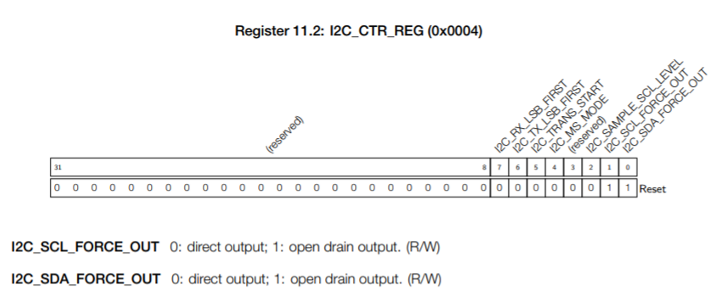
\includegraphics[width = 10cm]{images/reg_esp.png}
    \caption{ESP32 Register, ESP32 reference manual, page 292}
    \label{fig:reg_esp}
\end{figure}

We can probably force it into push-pull by switching these bits to 0.
\begin{lstlisting}[language=C++]
  uint32_t reg_value &= ~0x02;
  *((uint32_t*) 0x3FF53004 )  = reg_value;
\end{lstlisting}

This (AND NOT) operation changes the last bit 1 to 0.

This would allow faster I2C communication.

However,This actually changed the clock line to be driven by the ESP (the data cannot, because it is already driven by the camera). However, at some point in the I2C operation, the values of this register are reset and therefore this technique does not work… This may be a point of improvement but it requires to go further into the driver operations of the I2C communication. 

The explanation is that Wire.begin() calls i2cInit() in
\begin{lstlisting}
\arduino-esp32-master\cores\\esp32\esp32-hal-i2c.c
\end{lstlisting}which, notably does:

\begin{lstlisting}[language=C++]
i2c->dev->ctr.val = 0;
i2c->dev->ctr.ms_mode = 1;
i2c->dev->ctr.sda_force_out = 1 ;
i2c->dev->ctr.scl_force_out = 1 ;
i2c->dev->ctr.clk_en = 1;
\end{lstlisting}

Which obviously put sclForceOut to 1. However, I was careful to change the value after the init. But i2cInit is also called in case of an error:

\begin{lstlisting}[language=C++]
if(last_error == I2C_ERROR_BUSY) { // try to clear the bus
    if(i2cInit(i2c->num, i2c->sda, i2c->scl, 0)) {
        last_error = i2cProcQueue(i2c, NULL, timeOutMillis);
        }
    }
\end{lstlisting}

So it calls the init again which reset the communication and creates a delay at each loop when trying to put the bit to 0. 

On an oscilloscope we can also see that the "rest" state of the clock is low, instead of high previously. This means that changing the register value has indeed an effect. The ESP is then waiting for a high value which never happens and probably a watchdog creates a timeout that then triggers the error.

 The error is probably triggered because the pin is in a mode (probably INPUTPULLUP) that works well with open drain mode. When put in driven output, the pin does not respond correctly and the clock is not actually transmitted which creates the error and resets the I2C.

The I2C function that handles the pinmode is:
\begin{lstlisting}[language=C++]
i2c_err_t i2cAttachSCL(i2c_t * i2c, int8_t scl)
{
    if(i2c == NULL) {
        return I2C_ERROR_DEV;
    }
    digitalWrite(scl, HIGH);
    pinMode(scl, OPEN_DRAIN | PULLUP | INPUT | OUTPUT);
    pinMatrixOutAttach(scl, I2C_SCL_IDX(i2c->num), false, false);
    pinMatrixInAttach(scl, I2C_SCL_IDX(i2c->num), false);
    return I2C_ERROR_OK;
}
\end{lstlisting}

Further work could be done on understanding exactly why it happens and if that can be changed. The I2C frequency for the moment is about 650kHz so being able to push it to 1MHz might help.
However, it is also possible that the camera does not refresh high enough and therefore the communication is blocked by this bottleneck.

\appendix
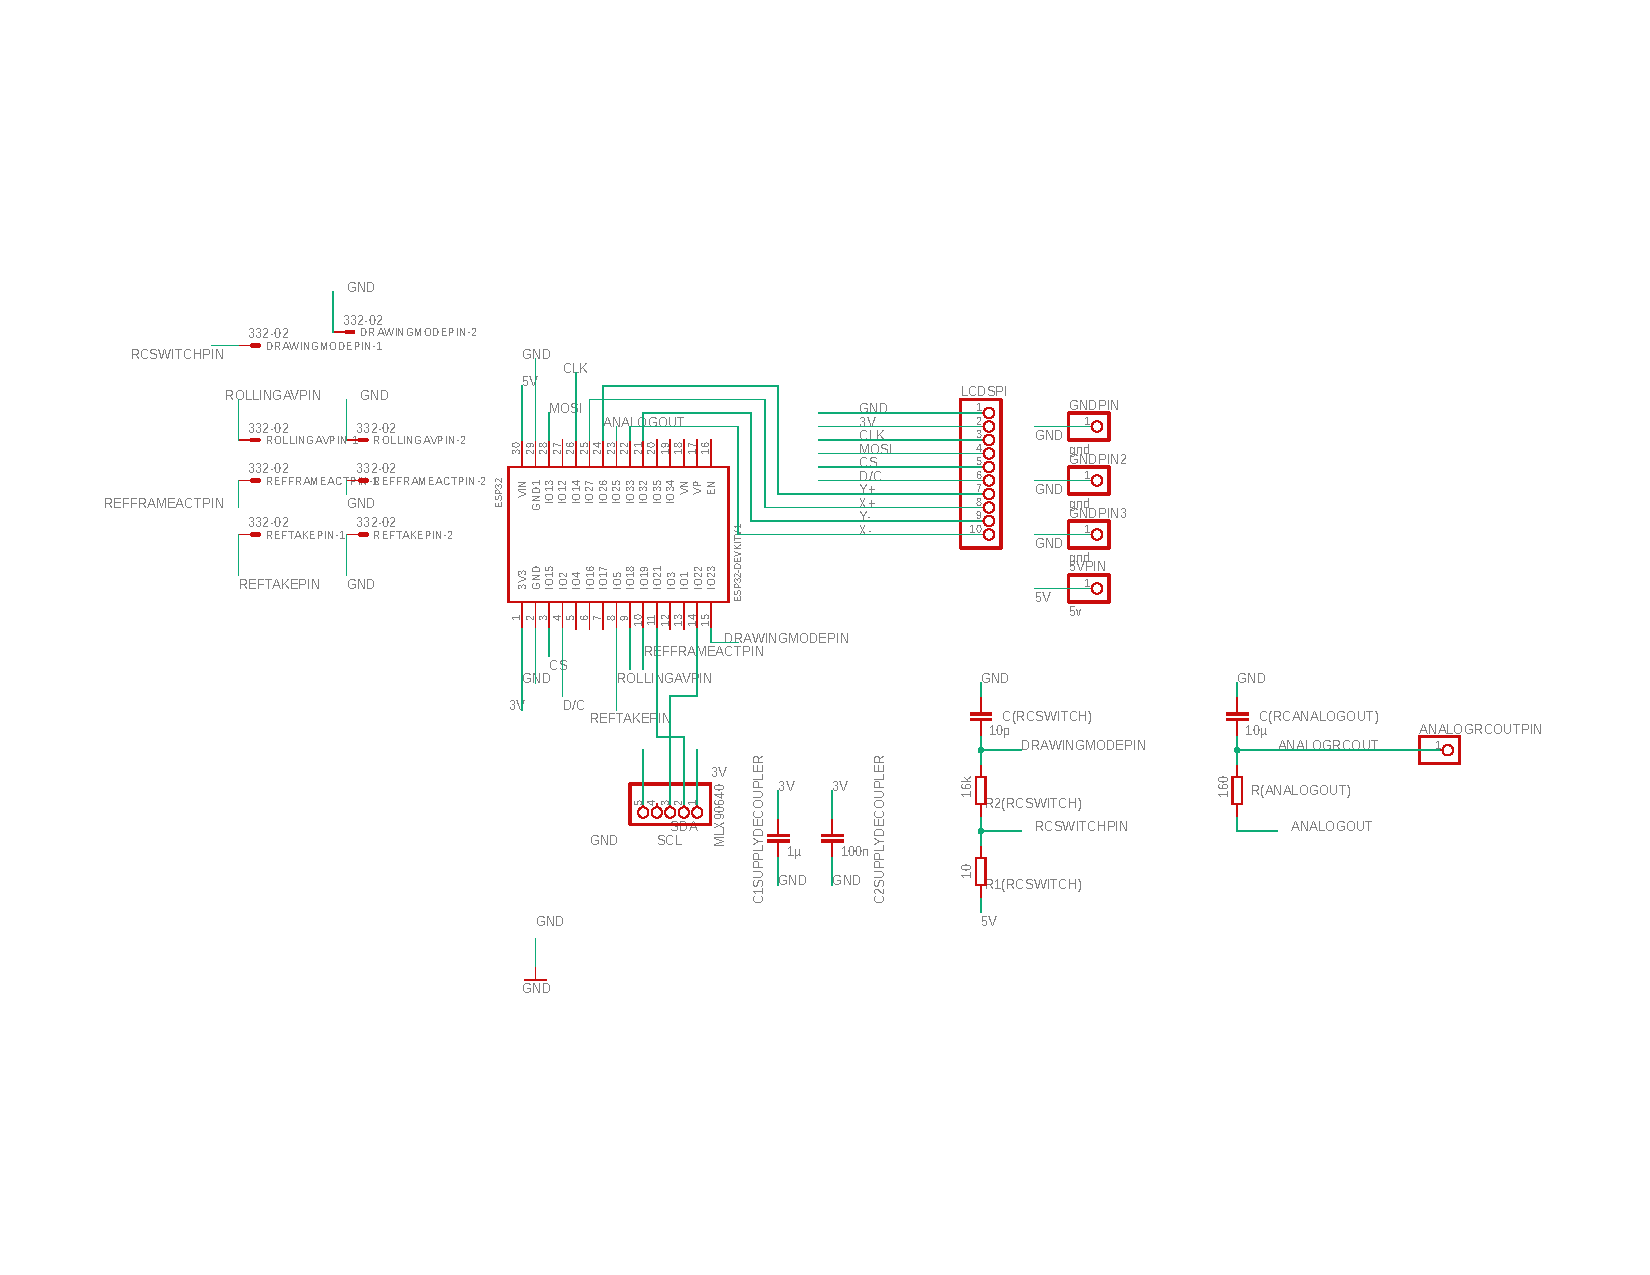
\includepdf[pagecommand = \section{PCB Schematic \label{schematic}}, angle = 270]{images/schematic}



\bibliographystyle{alpha}
\bibliography{biblio}

\end{document}